
\chapter{Dinámica de redes} \label{Ch:04}

En este capítulo se comienza el estudio de las vibraciones de los átomos alrededor de sus posiciones de equilibrio y sus efectos observables. Esta llamada \textit{dinámica de redes} es necesaria para explicar propiedades como: i) la conductividad térmica de los aislantes, ii) la dependencia en $T^3$ del calor específico a baja temperatura, iii) las energías de cohesión, iv) la dilatación térmica, v) la conductividad eléctrica \textit{finita} de los metales, vi) la reflectividad de los cristales iónicos, etc.


\section{Vibraciones de los cristales con base atómica}

Aquí se utilizará la llamada \textit{aproximación armónica} que consiste en aceptar que las desviaciones de las posiciones atómicas (respecto del equilibrio) son mucho menores que las distancias interatómicas 

\begin{equation}
	\rn (t) = \Rn + \Delta  \rn (t)  \quad \textit{con} \quad |\Delta \rn (t) | \ll |\rn (t)| \sim |\Rn|
\end{equation}
Esta aproximación equivale a decir que la fuerza elástica sobre un átomo es \textit{lineal} con los desplazamientos relativos $\Fn \propto \Delta \rn (t)$.

\subsection{La cadena lineal monoatómica}

El modelo es una cadena unidimensional de átomo de masa $M$ e interdistancia $a$ que puede servir para representar algunas de las vibraciones de un cristal tridimensional. Así, las vibraciones elásticas de un cristal cuando el vector de onda $\kn$ apunta en las direcciones [100], [110]  ó [111] en un cristal cúbico pueden suponerse unidimensionales en el sentido de que se necesita una sola coordenada, pues se espera que los planos de átomos perpendiculares $\kn$ se muevan en fase. 

\begin{figure}[h!] \centering
    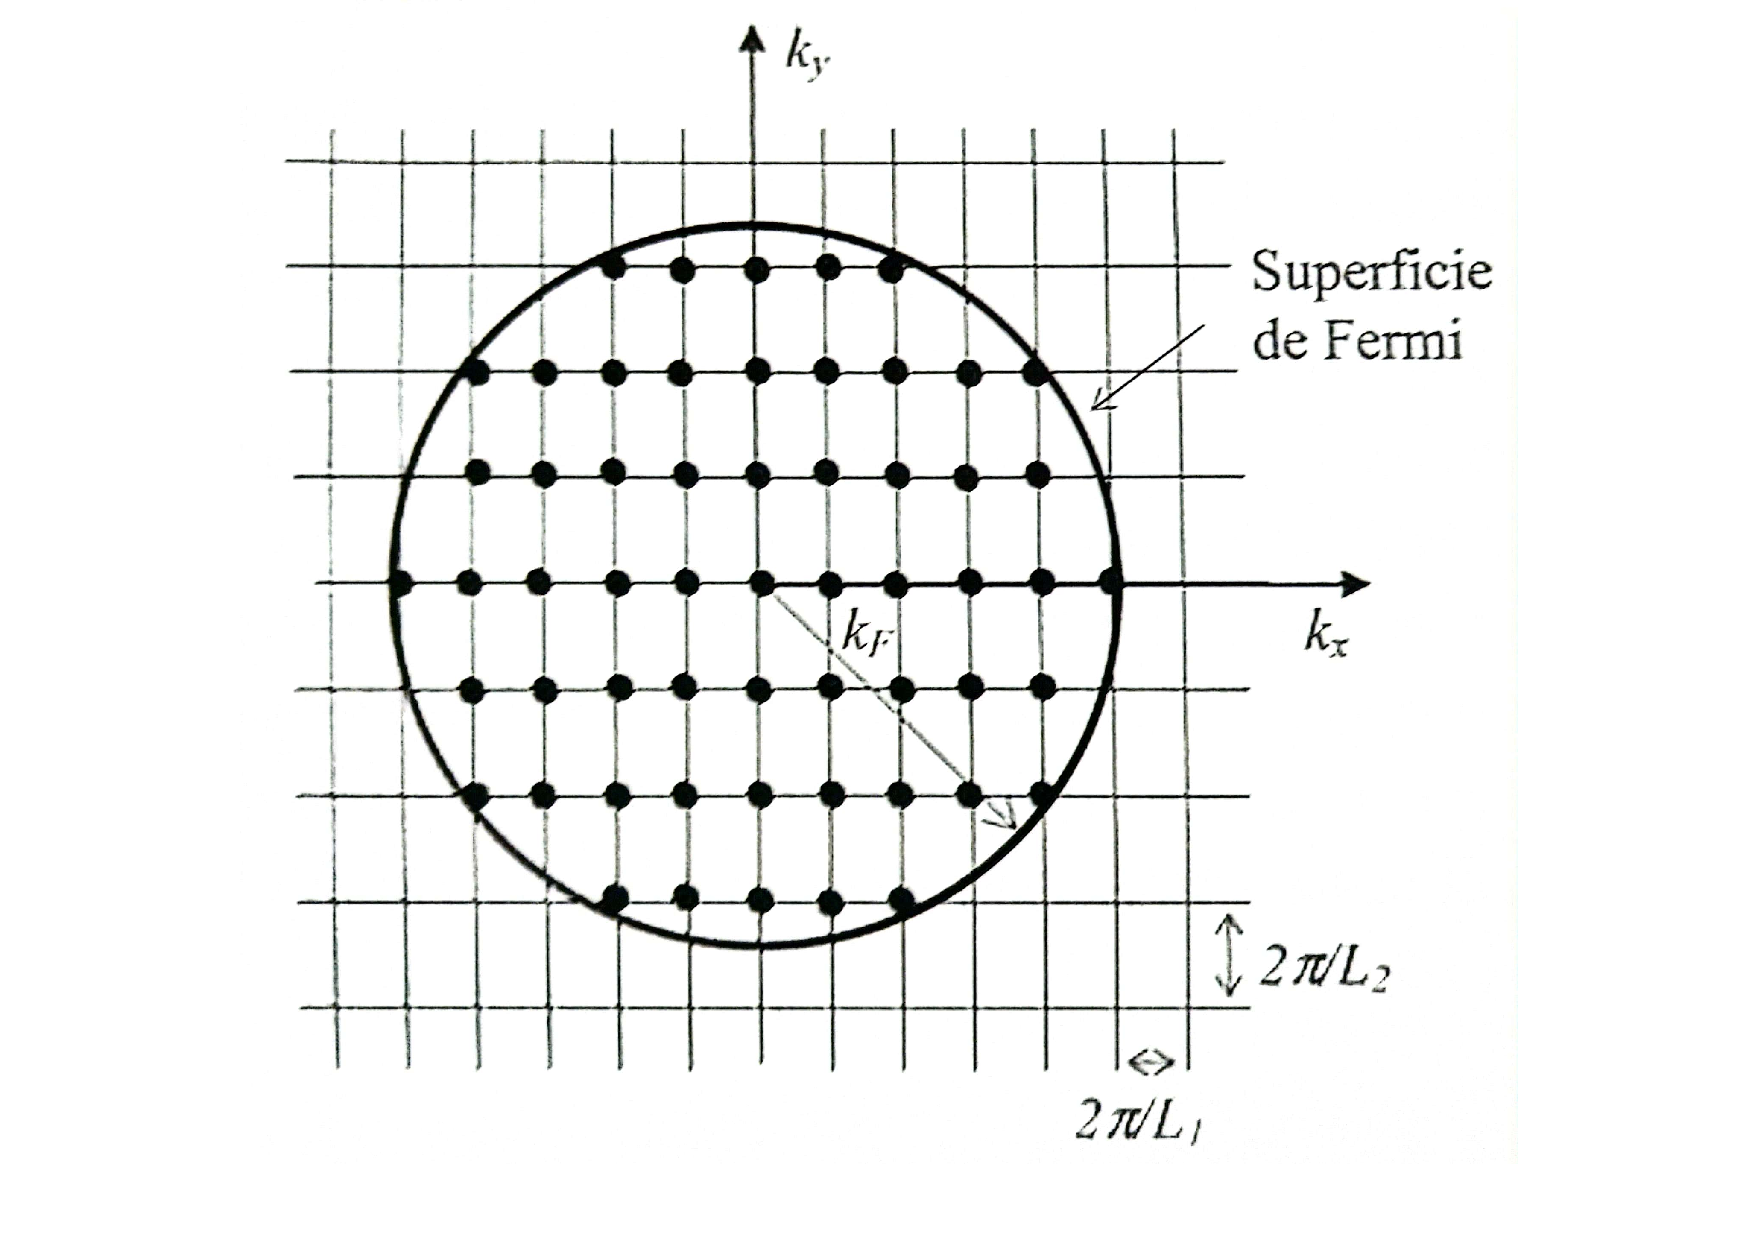
\includegraphics[scale=0.45]{Cuerpo/Ch_04/Fotos libro 1.pdf}
    \caption{Parámetro de red y posiciones de átomos de masa $M$ conectados por una fuerza de constante $C$ entre planos adyacentes. Los desplazamientos de los átomos se designan por $u_{s-1},u_{s},u_{s+1}$.}
    \label{Fig:04-01}
\end{figure}    

Denotando por $u_s$ la desviación del átomo (o plano) $s$ (ver figura \ref{Fig:04-01}), su ecuación del movimiento es

\begin{equation}
	M \derivadas{^2 u_s}{t^2} = F_s = - \parciales{U_{\text{arm}}}{u_s} \label{Ec:04-01-02}
\end{equation}
con 

\begin{equation}
	U_{\text{arm}} = \frac{1}{2} \sum_{s,l} \frac{C_l}{2} \parentesis{u_{s+l}-u_s}^2
\end{equation}
$C_l$ es la constante de fuerza entre dos átomos separados $la$. Esta expresión se justifica por la aproximación armónica citada. Si los desplazamientos son suficientemente pequeños el término dominante del desarrollo en serie de Taylor de la energía potencial es el cuadrático, pues el lineal no existe porque se exige $U_{\text{arm}}$ mínimo (derivada nula) en $u_s$. El factor $1/2$ que multiplica a la suma se introduce para no contar dos veces la misma interacción. 

Para simplificar se tendrían en cuenta aquí solo interacciones entre vecinos más próximos, es decir, $l=\pm 1$, con lo cual $C_\pm = C$ y 

\begin{equation}
	U_{\text{arm}} = \frac{C}{2} \sum_s \ccorchetes{\parentesis{u_{s+1}+u_s}^2+\parentesis{u_{s-1}-u_s}^2}
\end{equation}
y por tanto la fuerza total sobre $s$ 

\begin{equation}
	F_s = C (u_{s+1}-u_s) + C(u_{s-1}-u_s)
\end{equation}
Por la anisotropía de los sólidos, en general $C$ será diferente según la dirección en la que se producen las oscilaciones. 

Con esta aproximación, la ecuación del movimiento (\ref{Ec:04-01-02}) admite la solución armónica

\begin{equation}
	u_s = u_k e^{i(ksa-\omega t)}
\end{equation}
siempre que se verifique 

\begin{equation}
	\omega = \sqrt{\frac{4C}{M}} \left| \sin \parentesis{\frac{1}{2} k a} \right| \label{Ec:04-01-07}
\end{equation}
que es llamada la \textit{relación de dispersión} y cuya gráfica se muestra en la figura \ref{Fig:04-02}. Algunos puntos importantes son:

\begin{itemize}
	\item Hay simetría $k\rightarrow -k$.
	\item Hay periodicidad $k\rightarrow k+n2\pi/a=k+G$. La razón de que $k$ y $k+G$ sean equivalentes es que dan lugar a las mismas coordenadas atómicas, como se muestra con el ejemplo de la figura \ref{Fig:04-03}. Por la \textit{redundancia} existente en el espectro sólo consideramos los vectores de onda $k \in PZB$.
	\item La \textit{velocidad de grupo} $v_g = \D\omega / \D k$ se anula en $k=\pm \pi/a$. Observar que éstos precisamente los valores que satisfacen la condición de Bragg, por lo que parece como si la onda $k=\pi / a$ se reflejara internamente ($k \rightarrow -k$) para dar lugar a una \textit{onda estacionaria}.
	\item No pueden existir ondas viajeras con $\omega>2 (C/M)^{1/2}$.
	\item Para $ka\rightarrow 0 \approx a(C/M)^{1/2}k$, es decir, la \textit{la velocidad de fase} $c=\omega /k$ es constante, y es por lo que la relación de dispersión (\ref{Ec:04-01-07}) se denomina \textit{rama acústica}. $c=a \omega_{\max} /2$ es la velocidad del sonido en el cristal.
\end{itemize}


\begin{figure}[h!] \centering
    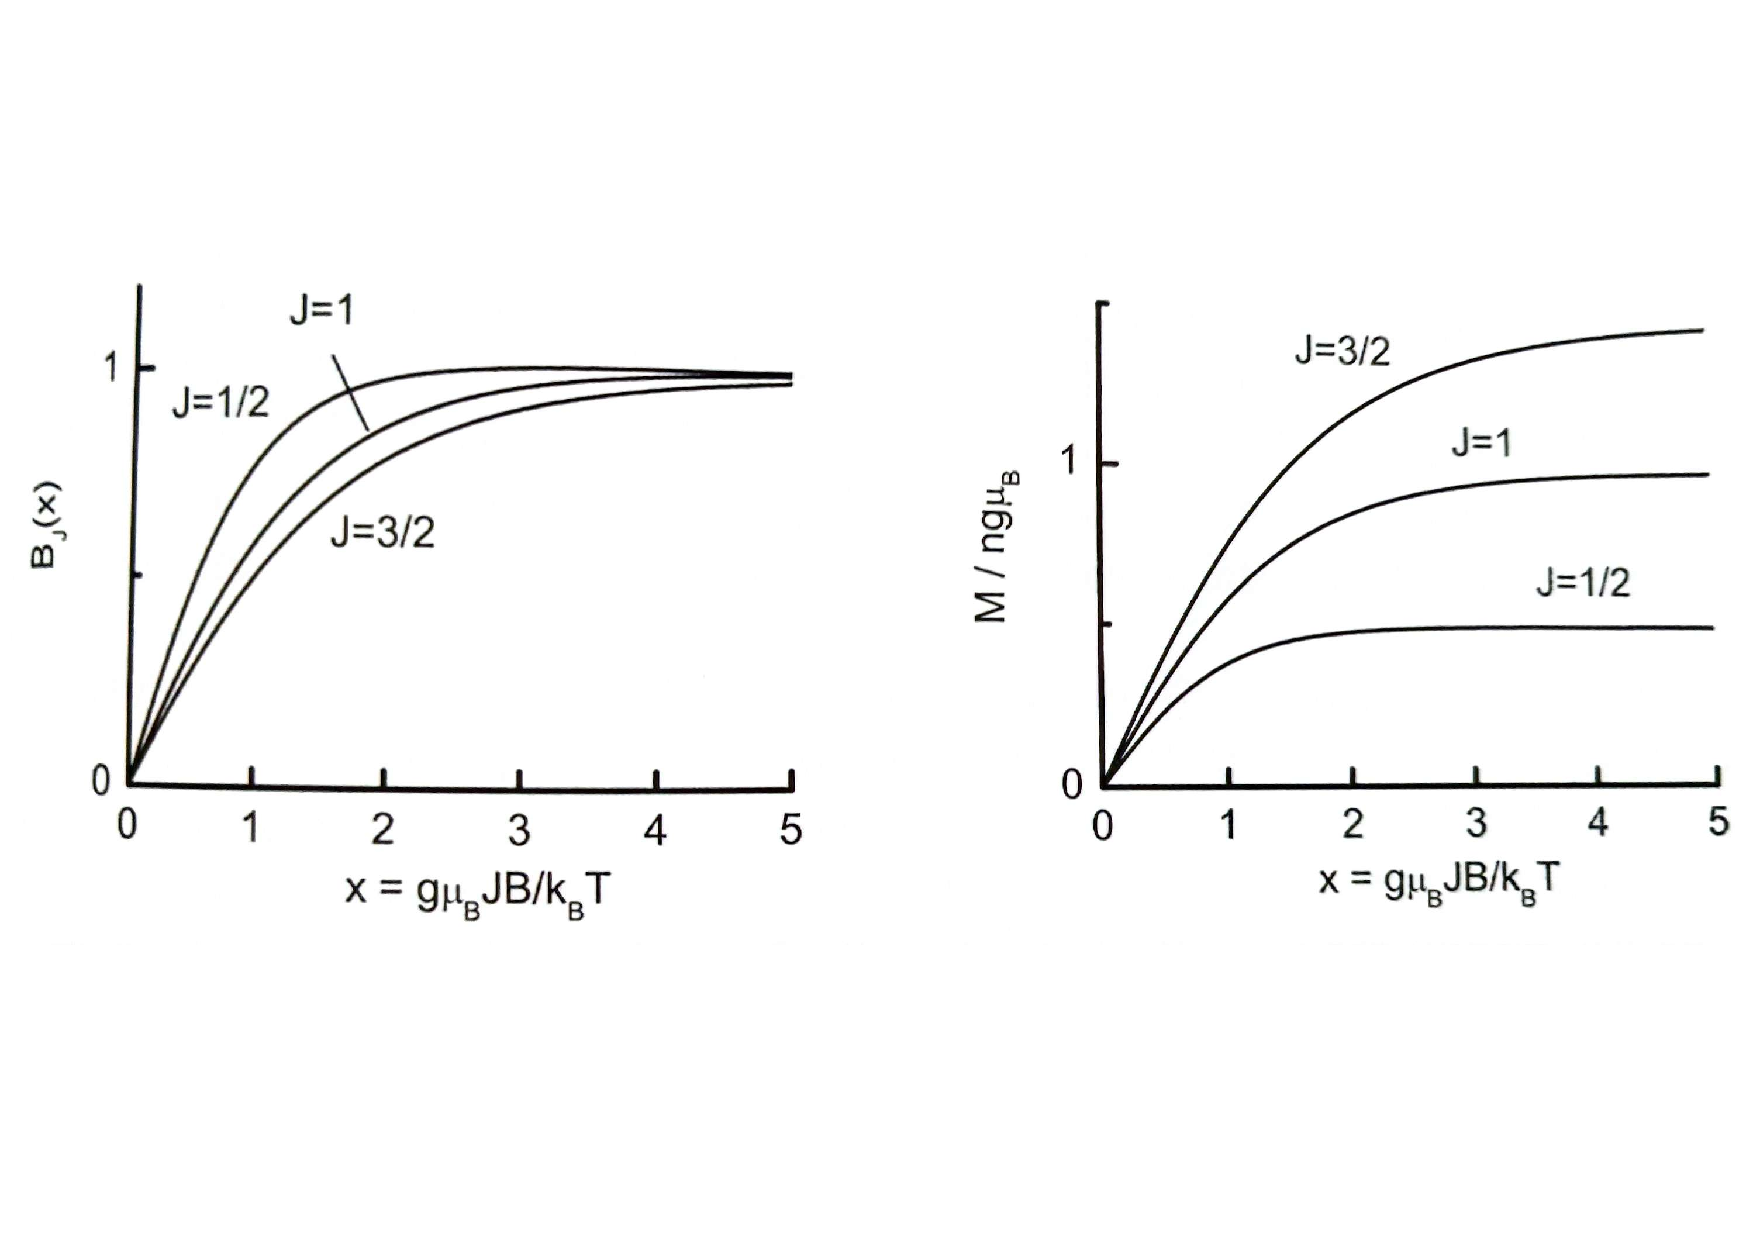
\includegraphics[scale=0.45]{Cuerpo/Ch_04/Fotos libro 2.pdf}
    \caption{Representación de la relación de dispersión de una cadena monoatómica de átomos de masa $M$ y constante de acoplamiento $C$. Observar que para $k\rightarrow 0$, $\omega \rightarrow k$}
    \label{Fig:04-02}
\end{figure}    

\begin{figure}[h!] \centering
    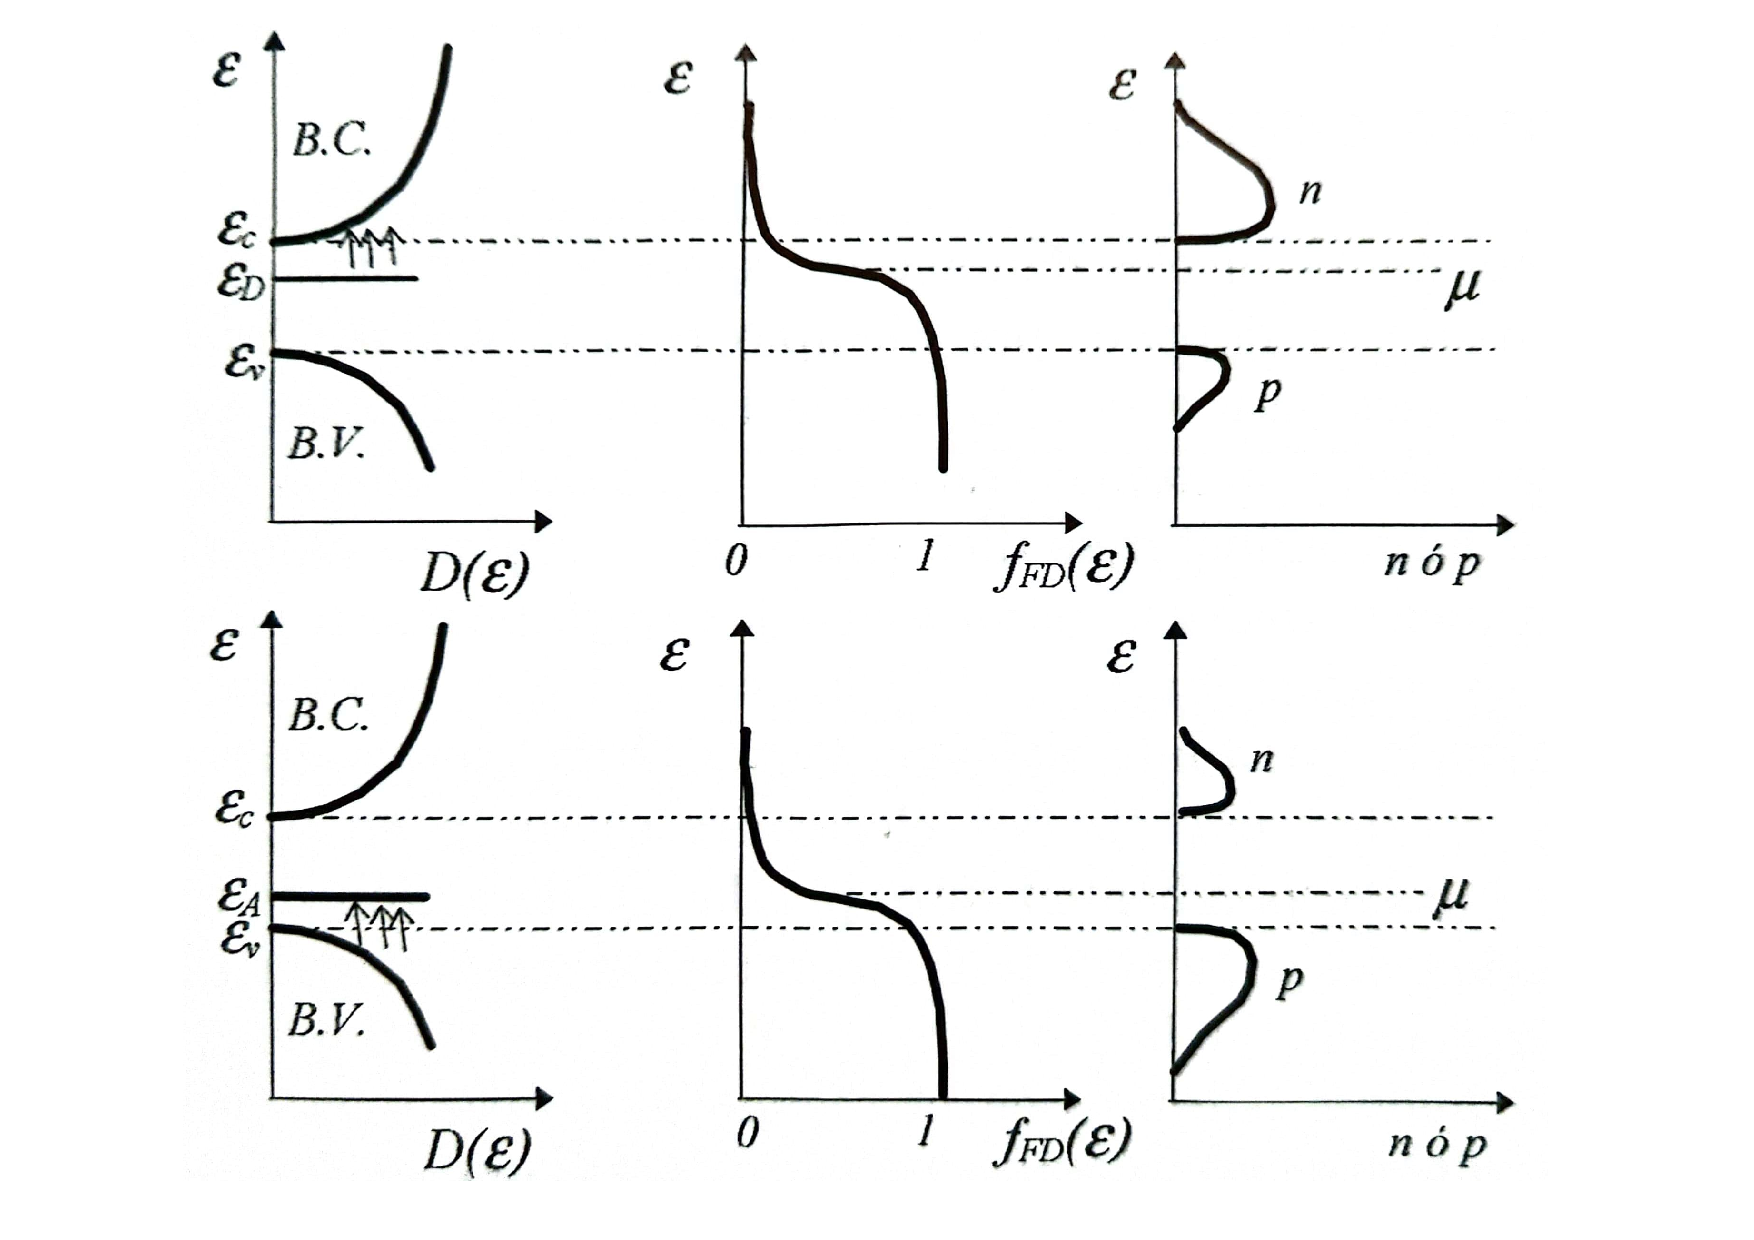
\includegraphics[scale=0.45]{Cuerpo/Ch_04/Fotos libro 3.pdf}
    \caption{Ejemplo de ondas con distancia longitud de onda que sin embargo representan el mismo estado de movimiento de los átomos.}
    \label{Fig:04-03}
\end{figure}    

\subsection{Cristales monoatómicoos tridimensionales}

En este caso, los átomos ocupan posiciones $\rn(t) = \Rn + \un (\Rn,t)$. Si llamamos a $\phi$ al potencial de interacción entre dos átomos, la \textit{aproximación armónica} nos permite aproximar la energía total por un desarrollo en serie a segundo orden:

\begin{equation}
	U_{\text{arm}} = \frac{1}{4} \sum_{\Rn,\Rn'} \ccorchetes{\un(\Rn)-\un(\Rn')} \Phi \ccorchetes{\un(\Rn)-\un(\Rn')} \label{Ec:04-01-08}
\end{equation}
con $\Phi_{ij}=\partial^2 \phi / \partial x_i \partial x_j$, siendo $x_i(t) = R_i + u_i (\Rn,t) \ (i,j=1,2,3)$. Equivalentemente (\ref{Ec:04-01-08}) se puede escribir como:

\begin{equation}
	U_{\text{arm}} = \frac{1}{4} \sum_{\Rn,\Rn'}\un(\Rn) D(\Rn-\Rn' ) \un(\Rn') \label{Ec:04-01-09}
\end{equation}
donde 

\begin{equation}
	 D(\Rn-\Rn' ) = \delta_{\Rn \Rn'} \sum_{\Rn''} \Phi (\Rn- \Rn'') - \Phi (\Rn - \Rn')
\end{equation}
es una matriz que contiene las interacciones entre pares de átomos. La {\bf ecuación dinámica} es

\begin{equation}
 	M \derivadas{\un (\Rn)}{t^2} =  - \parciales{U_\text{arm}}{\un (\Rn)} = \sum_{\Rn'} D (\Rn-\Rn') \un (\Rn') \label{Ec:04-01-11}
\end{equation}
que admite soluciones de la forma

\begin{equation}
	\un (\Rn,t) = \epsilonn (\Rn,t) e^{i(\kn \cdot \Rn - \omega t)}  \label{Ec:04-01-12}
\end{equation}
donde $\epsilonn(\kn)$ es el \textit{vector de polarización}. Al sustituir  (\ref{Ec:04-01-12}) en (\ref{Ec:04-01-11}) se ve que la condición de existencia de solución es 

\begin{equation}
	D(\kn) \epsilonn (\kn) = M \omega^2 (\kn) \epsilonn \kn \label{Ec:04-01-13}
\end{equation}
donde $D(\kn) = \sum_\Rn D(\Rn) e^{i \kn \cdot \Rn}$ es la llamada \textit{matriz dinámica}, que se puede ver que es real y simétrica. Esto garantiza la existencia de \textit{tres} soluciones a (\ref{Ec:04-01-13}) que verifican $\epsilonn_i (\kn) \cdot \epsilonn_j (\kn) = \delta_{ij}$, ($i,j=1,2,3$), y que se denominan \textit{ramas acústicas} por verificarse en ellas que $\omega_i (\kn) \approx c_i (\kn)k$ para $ka\ll 1$. Dado un $\kn$, los vectores $\epsilonn$ no tienen en general que ser paralelos o perpendiculares a $\kn$. Por eso sólo se puede hablar aproximadamente de \textit{polarización longitudinal} o \textit{transversal}. A pesar de ello, los tres modos posibles para cada $\kn$ se denominan \textit{acústica longitudinal} (LA) y \textit{acústicos transversales} (TA). El resto de las propiedades coinciden con las del caso unidimensional.

\section{Vibraciones de cristales con base diatómica}

\subsection{La cadena lineal diatómica}

El modelo es una cadena unidimensional con base diatómica. Los átomos de la base se distinguirán por tener masa distinta (véase \ref{Fig:04-04}), aunque sería equivalente distinguirlos por sus acoplamientos. Como antes, este modelo podría representar vibraciones de cristales reales en direcciones particulares. Las ecuaciones del movimiento, admitiendo interacción sólo a vecinos más próximos y una única constante de fuerza $C$ son

\begin{equation*}
	M_1 \derivadas{^2 u_s}{t^2} = C(v_s - u_s) + C(v_{s-1}-u_s)
\end{equation*}
\begin{equation}
	M_2 \derivadas{^2 v_s}{t^2} = C(u_{s+1} - v_s) + C(u_{s}-v_s) \label{Ec:04-02-01}
\end{equation}

\begin{figure}[h!] \centering
    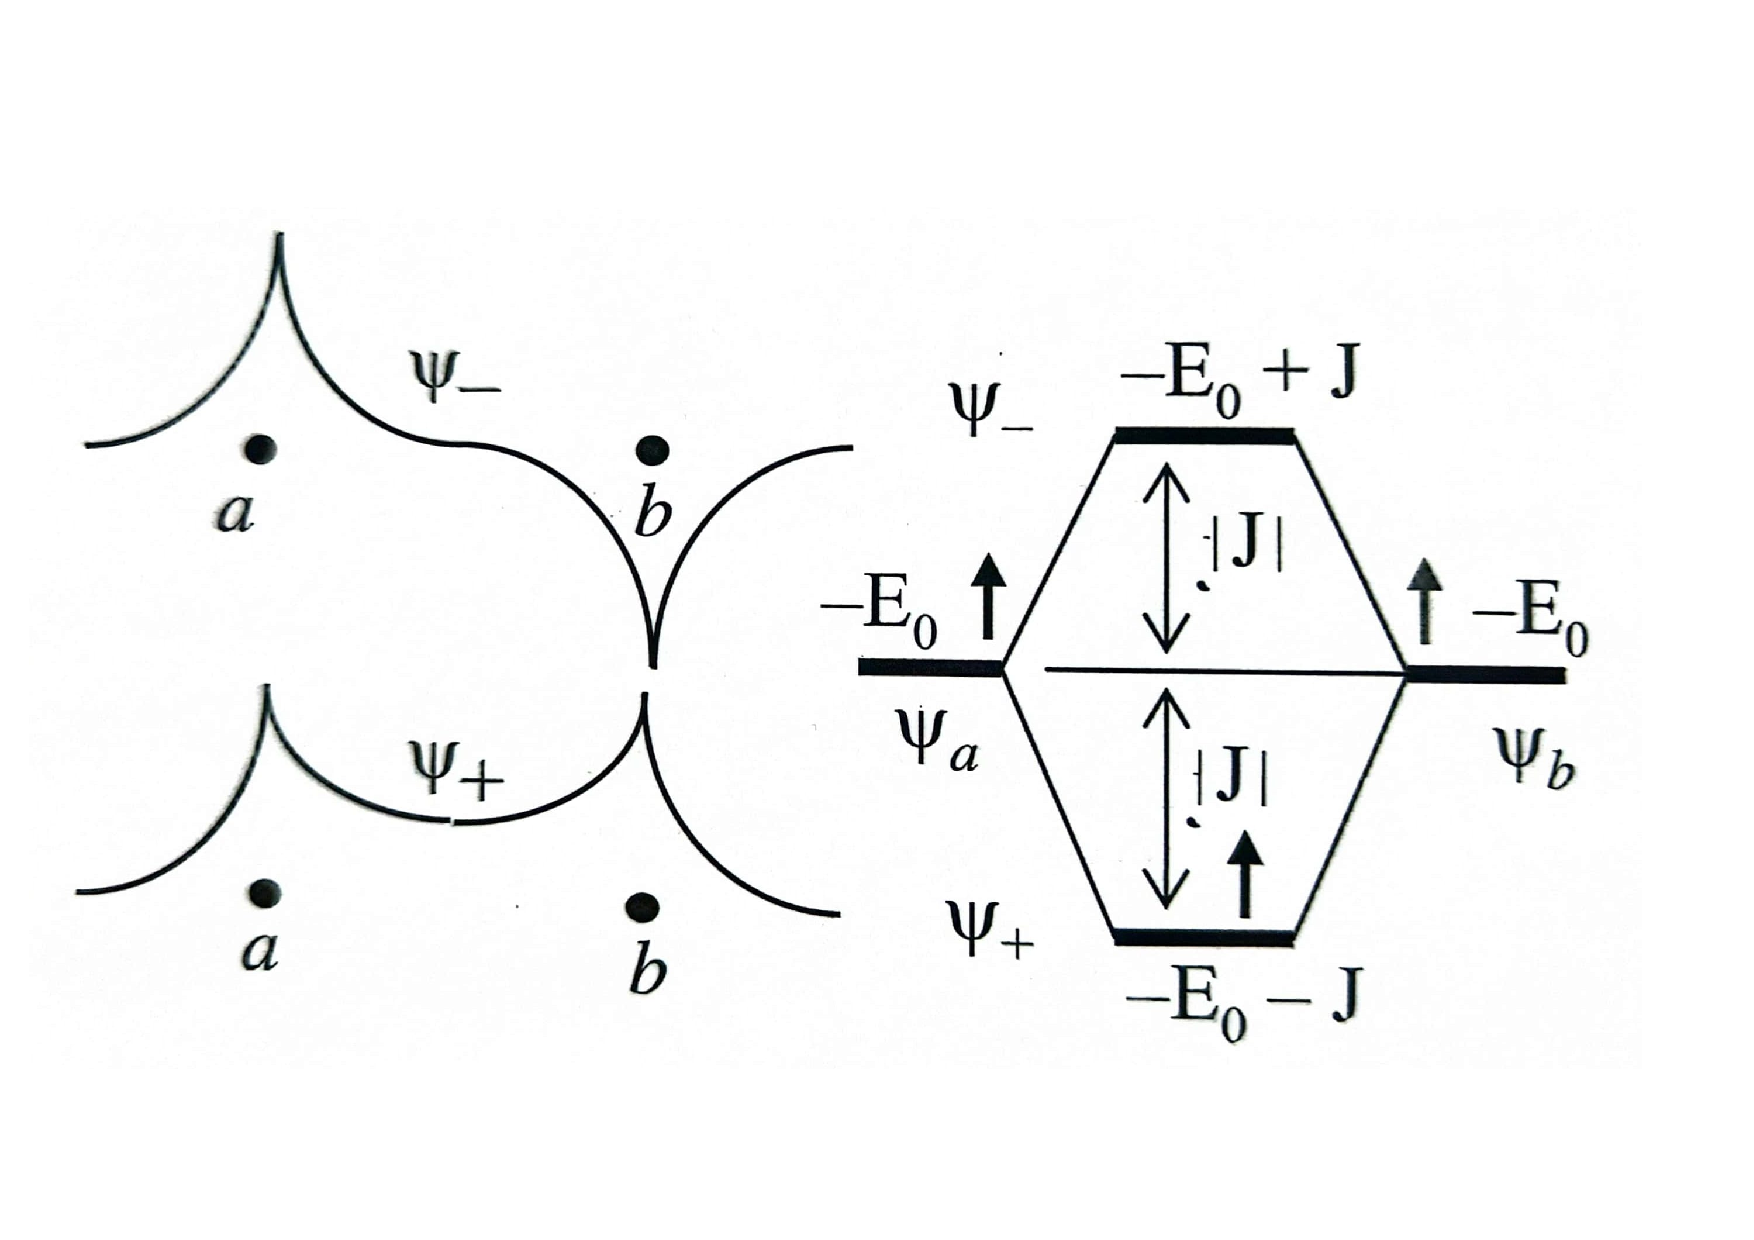
\includegraphics[scale=0.4]{Cuerpo/Ch_04/Fotos libro 4.pdf}
    \caption{Parámetro de red y posiciones de átomos 1 (masa $M_1$) y 2 (masa $M_2$) conectados por una fuerza de constante $C$ entre planos adyacentes. Los desplazamientos de los átomos 1 se designan por $u$ y los átomos 2 por $v$.}
    \label{Fig:04-04}
\end{figure}    

Una solución en modos normales, permitiendo amplitudes distintas para $M_1$ y para $M_2$ es 

\begin{equation}
	u_s = u_k e^{i(ksa-\omega  t)} \tquad v_s = v_k e^{i(ksa-\omega t)} \label{Ec:04-02-02}
\end{equation}
Al sustituir (\ref{Ec:04-02-01}) y (\ref{Ec:04-02-02}) se encuentra 



\begin{figure}[h!] \centering
    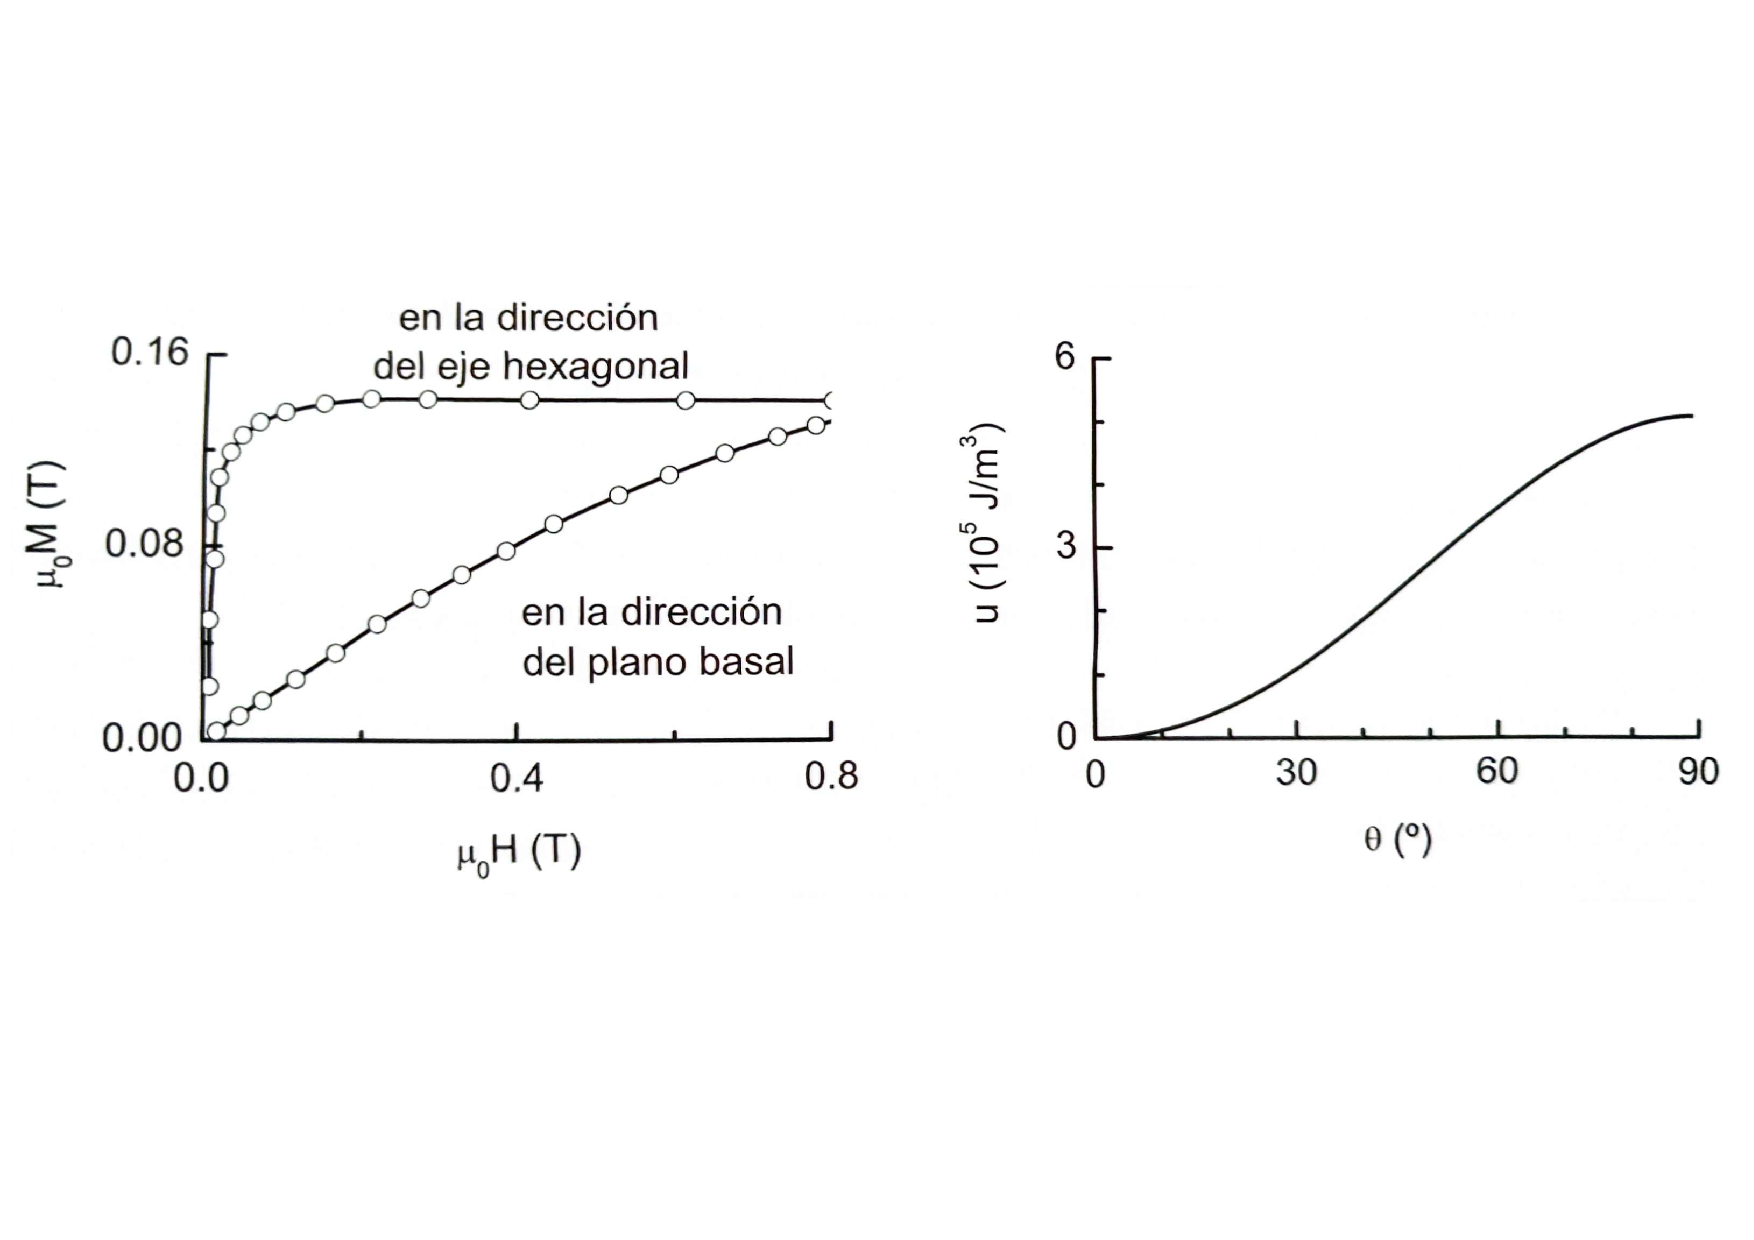
\includegraphics[scale=0.5]{Cuerpo/Ch_04/Fotos libro 5.pdf}
    \caption{Representación de la relación de dipsersión de una cadena diatómica de átomos de masas $M_1$ y $M_2$ y constante de acoplamiento $C$. Observar que para la rama óptica $\omega \rightarrow \text{cte} \neq 0$ cuando $k\rightarrow 0$.}
    \label{Fig:04-05}
\end{figure}    

\begin{figure}[h!] \centering
    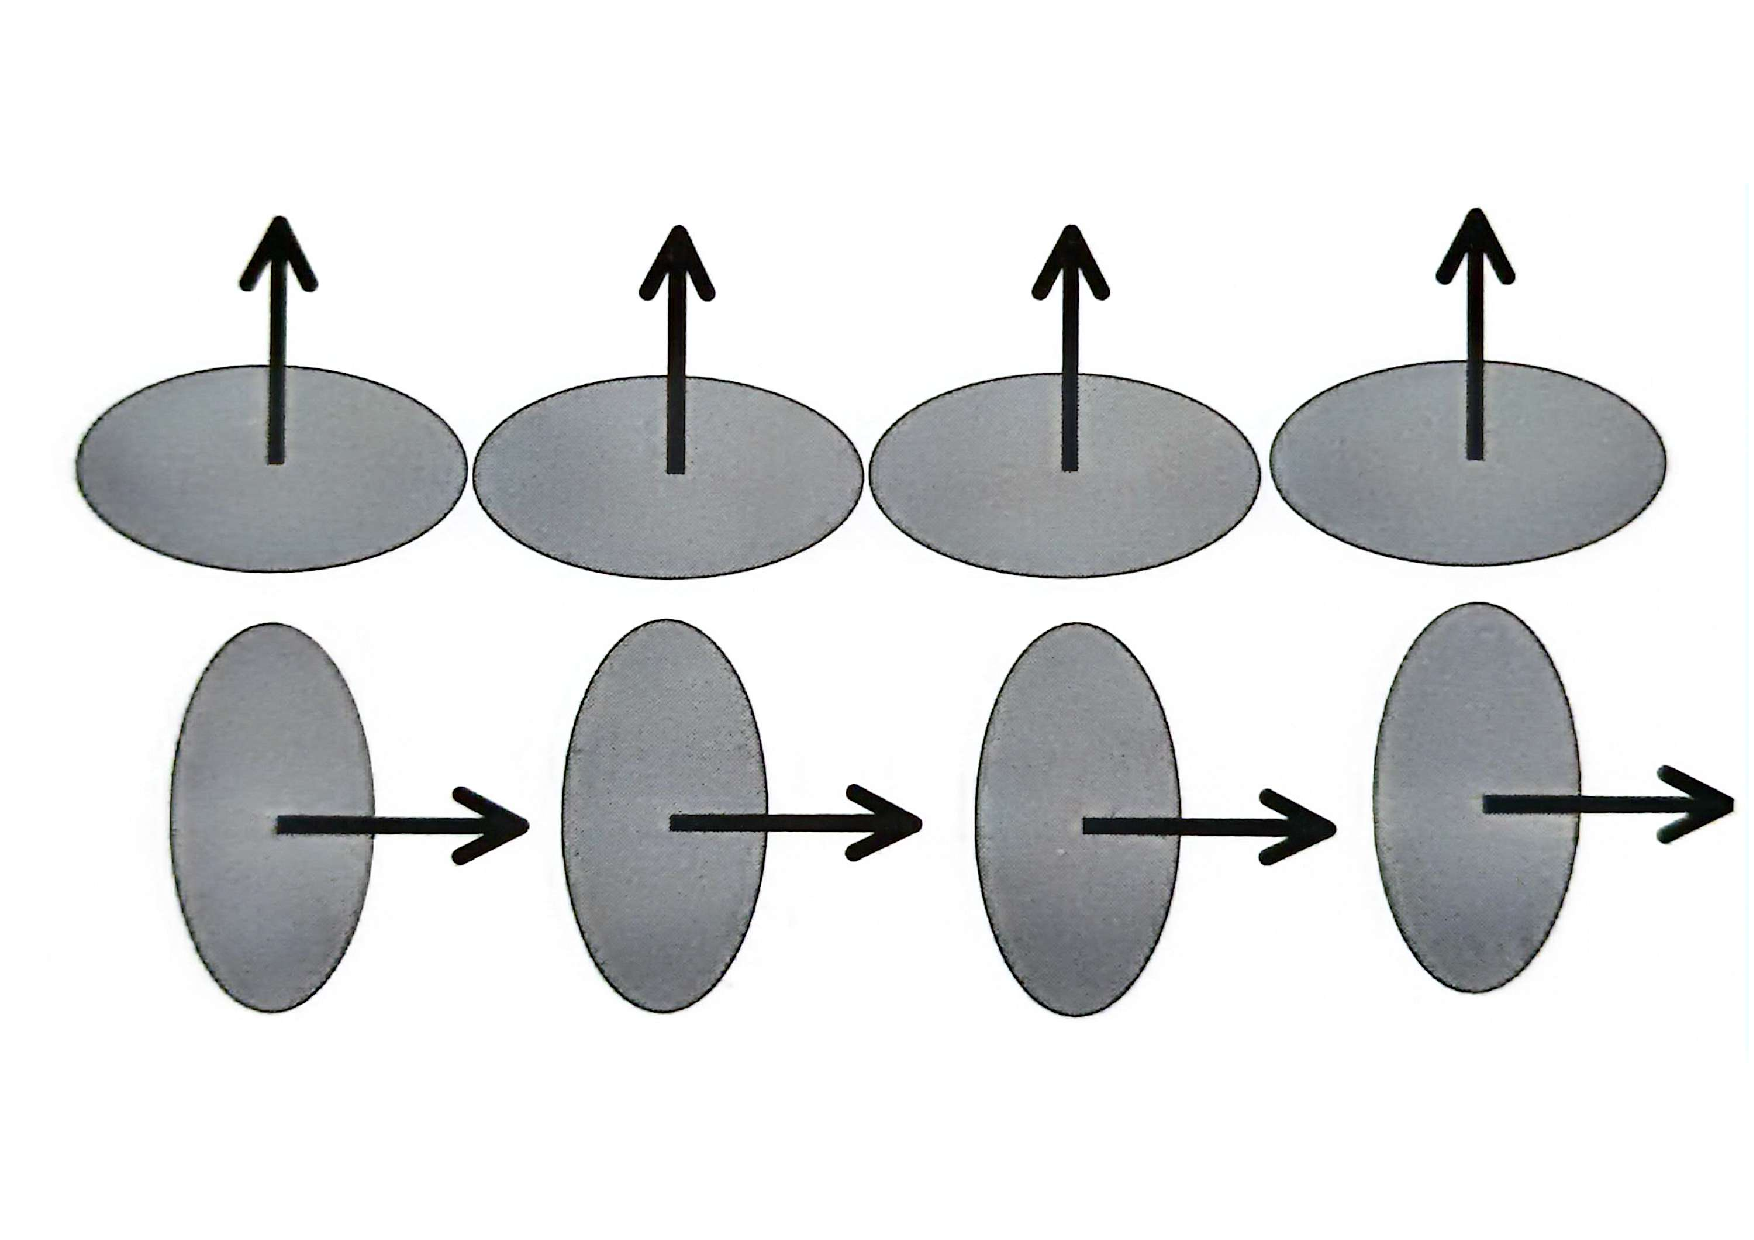
\includegraphics[scale=0.5]{Cuerpo/Ch_04/Fotos libro 6.pdf}
    \caption{Modos óptico y acústica en una cadena diatómica. El desplazamiento atómico respecto a la posición de equilibrio se representa verticalmente.}
    \label{Fig:04-06}
\end{figure}    

\subsection{Cristales tridimensionales poliatómicos}

\begin{figure}[h!] \centering
    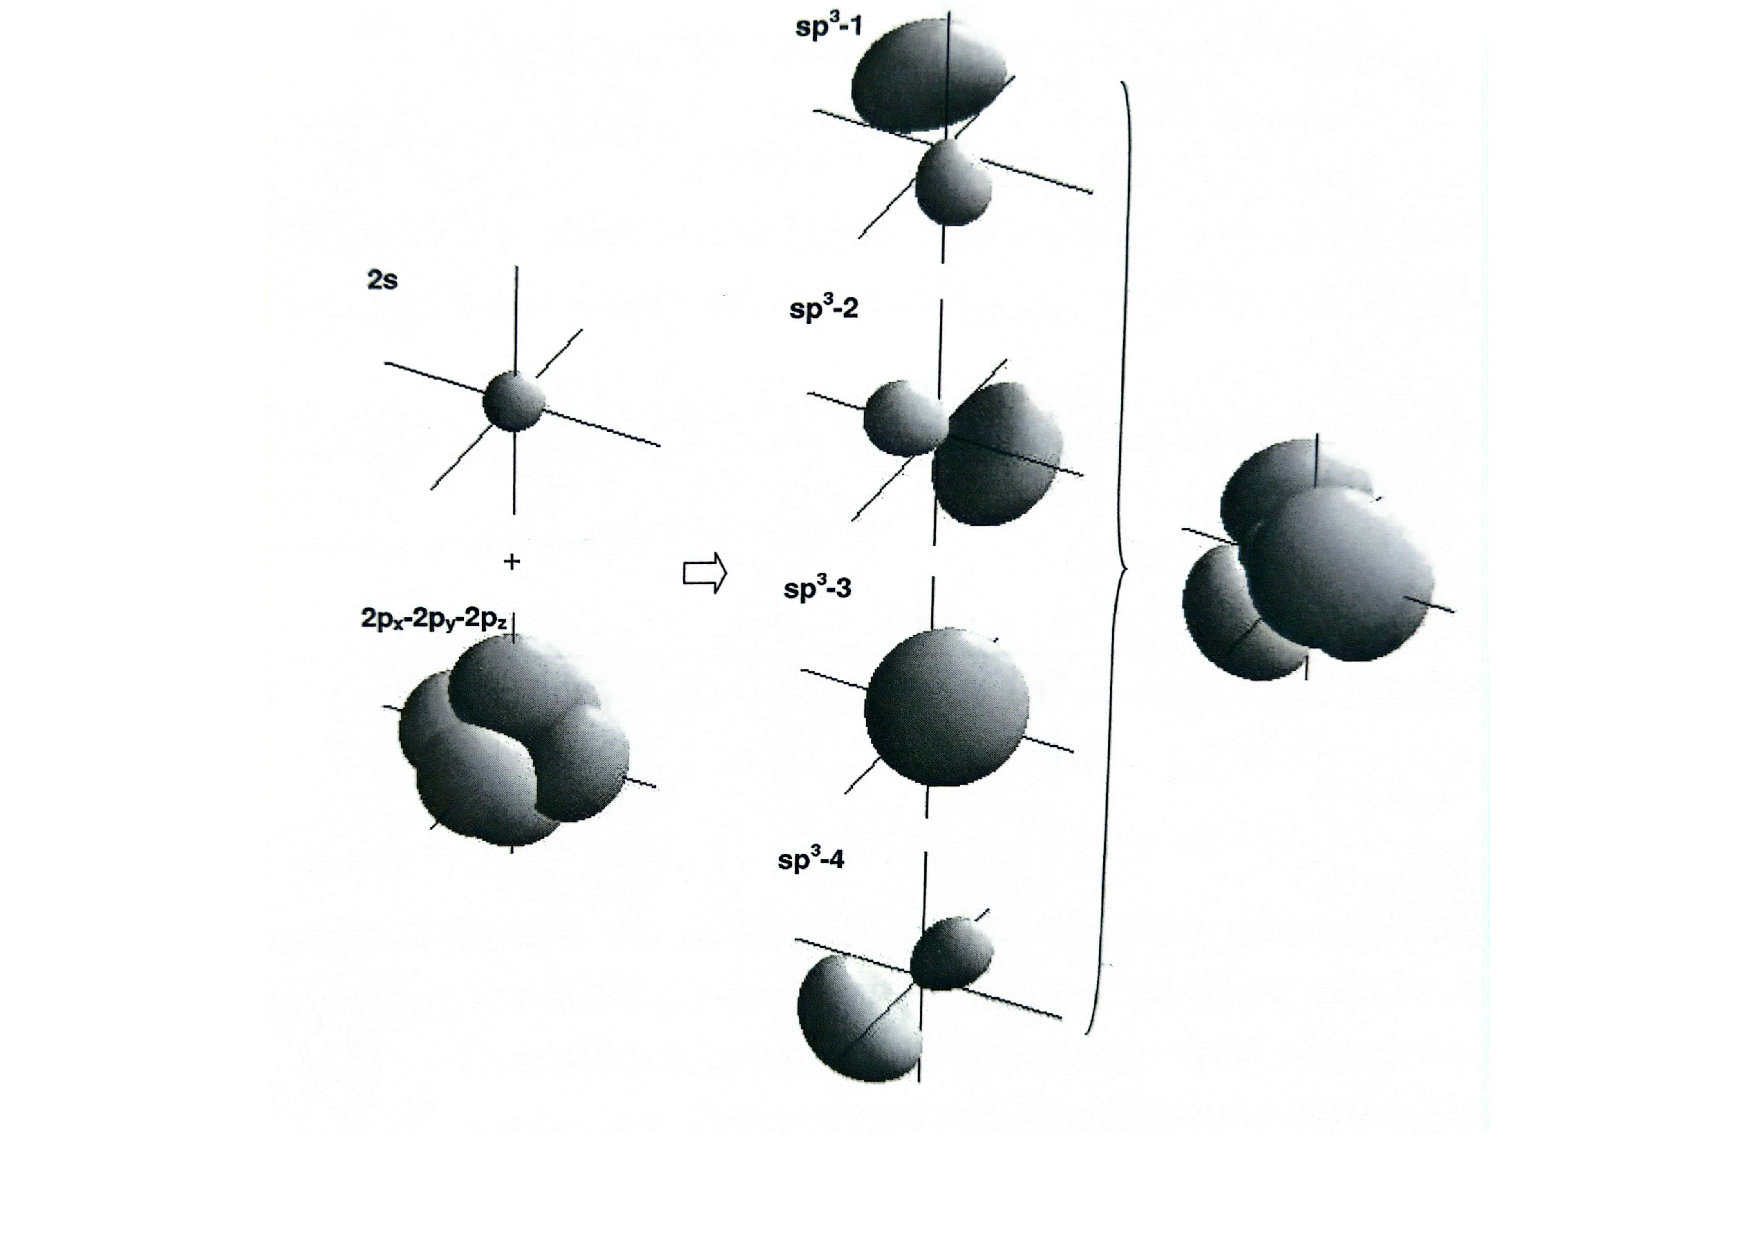
\includegraphics[scale=0.5]{Cuerpo/Ch_04/Fotos libro 7.pdf}
    \caption{Ejemplos de relación de dispersión experiental $\omega (\kn)$. En el eje horizontal se representa $\kn/\kn_{\max}$ para distintas direcciones, y en los ejes verticales la frecuencia $\omega/2\pi$ en undiades de $10^{12}$ Hz.}
    \label{Fig:04-07}
\end{figure}    



\section{Fonones}

\subsection{Cuantización de las ondas elásticas}

\subsection{Espectroscopía de fonones}


\section{Vibraciones de los cristales iónicos}
\begin{figure}[h!] \centering
    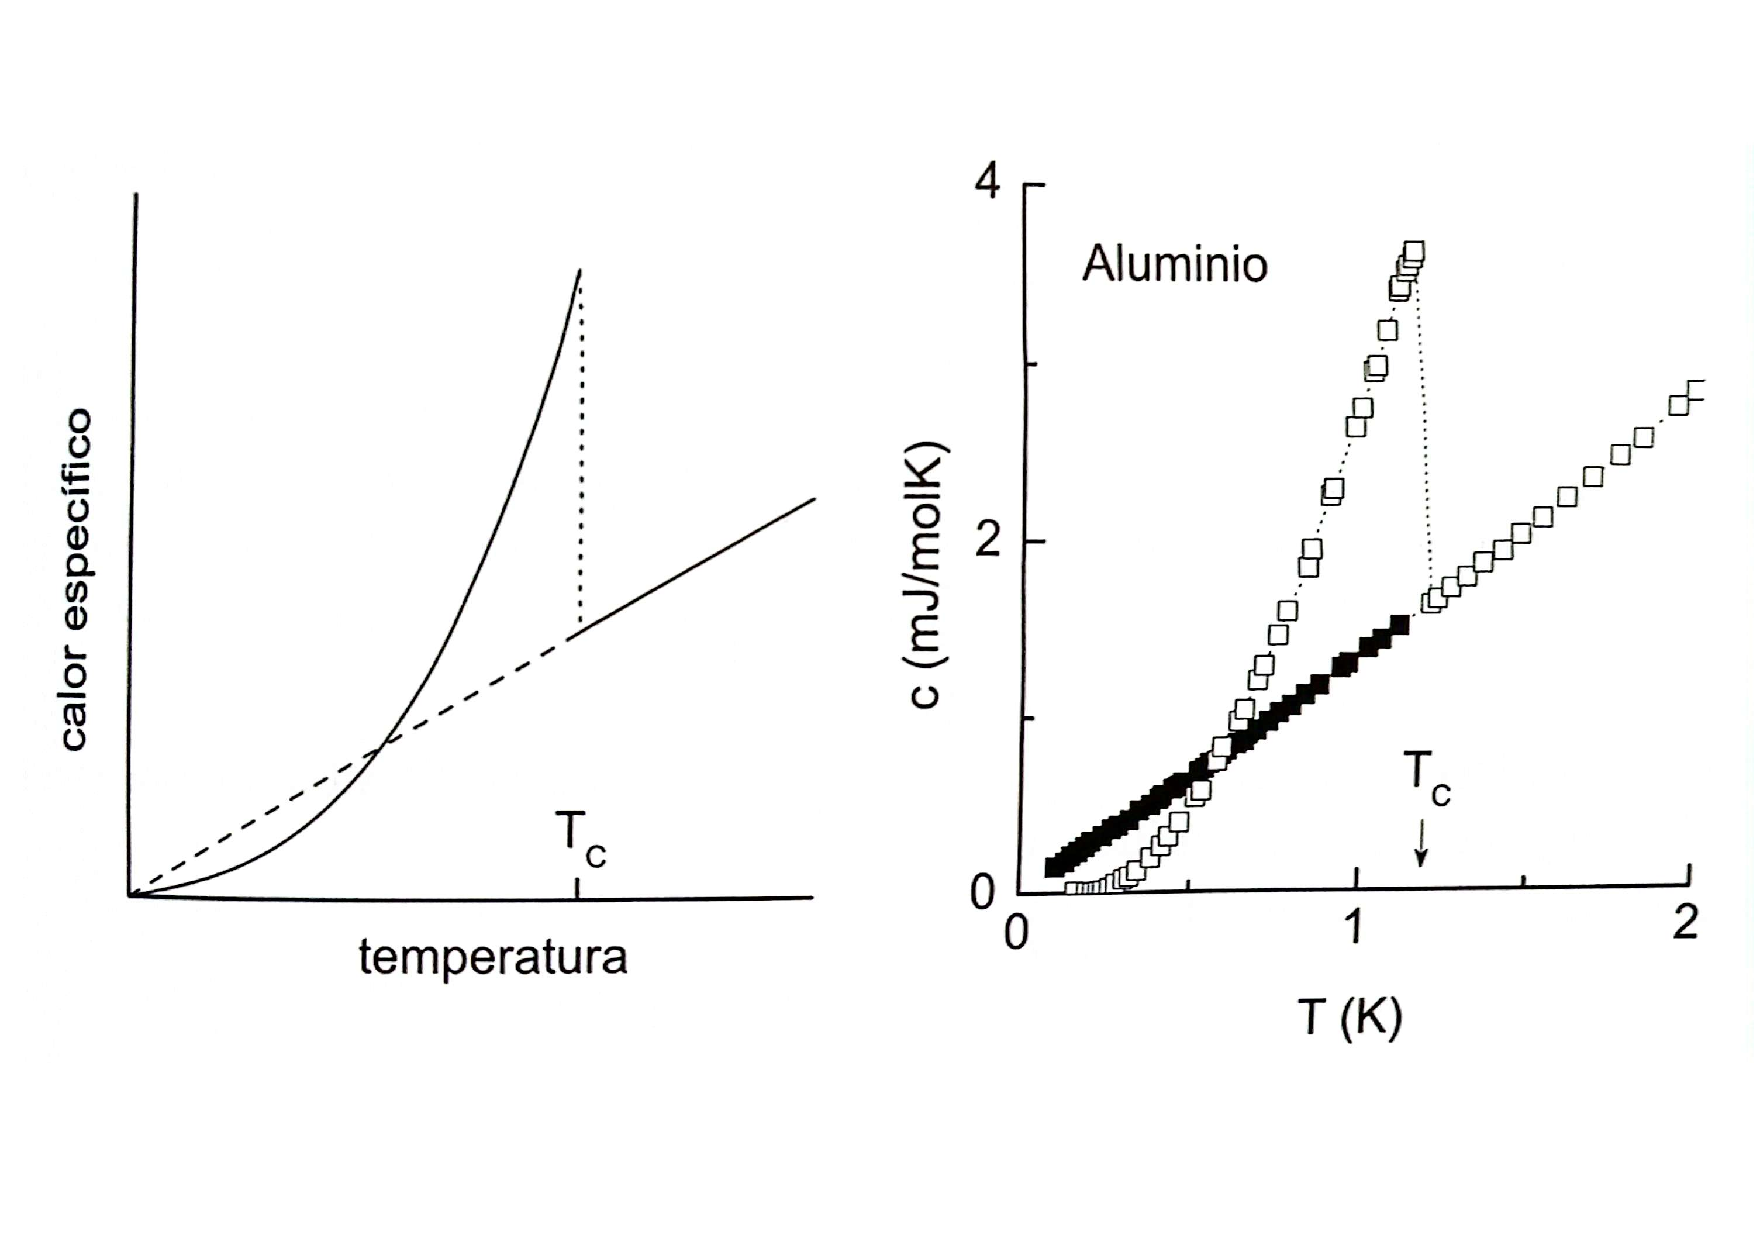
\includegraphics[scale=0.5]{Cuerpo/Ch_04/Fotos libro 8.pdf}
    \caption{(a) Dependencia con la frecuencia de la permitividad eléctrica relativa en cristales iónicos. (b) reflectividad de algunos cristales iónicos para longitudes de odna en el rango infrarrojo.}
    \label{Fig:04-08}
\end{figure}    
